\documentclass{article}
\usepackage{tikz}

\begin{document}

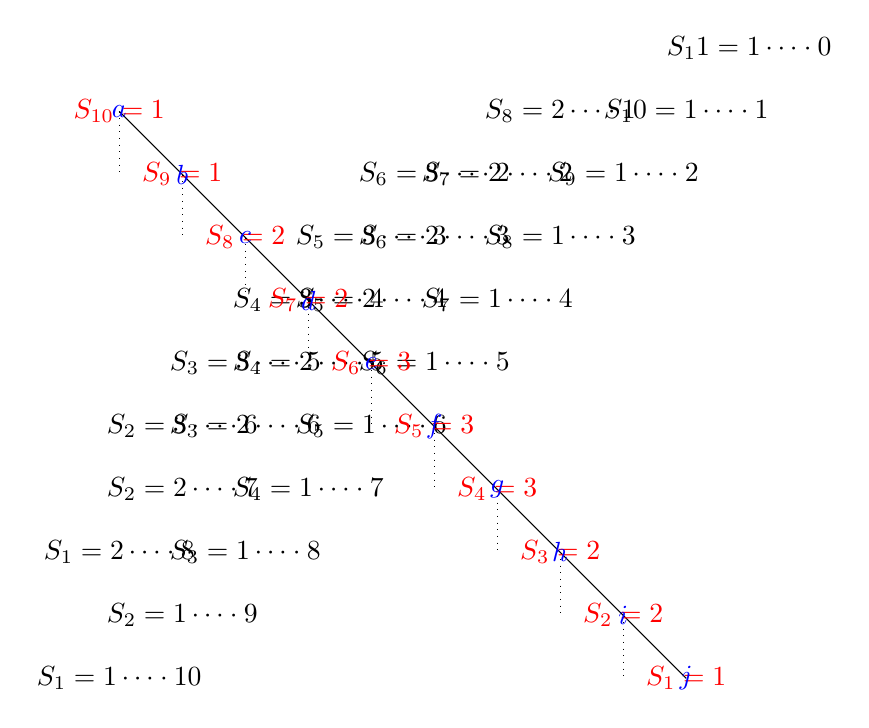
\begin{tikzpicture}[scale=0.8]
    % Nodes for the sequence S_j
    \foreach \j [count=\i] in {10,9,...,0} {
        \node at (\i,-\j) {$S_\i = 1 \cdots \cdot \j$};
    }
    \foreach \j [count=\i from 1] in {8,7,...,1} {
        \node at (\i,-\j) {$S_\i = 2 \cdots \cdot \j$};
    }
    \foreach \j [count=\i from 2] in {6,5,...,2} {
        \node at (\i,-\j) {$S_\i = 3 \cdots \cdot \j$};
    }

    % Lines connecting the nodes
    \draw (1,-1) -- (2,-2);
    \draw (2,-2) -- (3,-3);
    \draw (3,-3) -- (4,-4);
    \draw (4,-4) -- (5,-5);
    \draw (5,-5) -- (6,-6);
    \draw (6,-6) -- (7,-7);
    \draw (7,-7) -- (8,-8);
    \draw (8,-8) -- (9,-9);
    \draw (9,-9) -- (10,-10);

    % Dotted lines
    \draw[dotted] (1,-1) -- (1,-2);
    \draw[dotted] (2,-2) -- (2,-3);
    \draw[dotted] (3,-3) -- (3,-4);
    \draw[dotted] (4,-4) -- (4,-5);
    \draw[dotted] (5,-5) -- (5,-6);
    \draw[dotted] (6,-6) -- (6,-7);
    \draw[dotted] (7,-7) -- (7,-8);
    \draw[dotted] (8,-8) -- (8,-9);
    \draw[dotted] (9,-9) -- (9,-10);

    % Labels for the sequence S_j
    \node[red] at (1,-1) {$S_{10}=1$};
    \node[red] at (2,-2) {$S_{9}=1$};
    \node[red] at (3,-3) {$S_{8}=2$};
    \node[red] at (4,-4) {$S_{7}=2$};
    \node[red] at (5,-5) {$S_{6}=3$};
    \node[red] at (6,-6) {$S_{5}=3$};
    \node[red] at (7,-7) {$S_{4}=3$};
    \node[red] at (8,-8) {$S_{3}=2$};
    \node[red] at (9,-9) {$S_{2}=2$};
    \node[red] at (10,-10) {$S_{1}=1$};

    % Labels for the sequence S_j
    \node[blue] at (1,-1) {$a$};
    \node[blue] at (2,-2) {$b$};
    \node[blue] at (3,-3) {$c$};
    \node[blue] at (4,-4) {$d$};
    \node[blue] at (5,-5) {$e$};
    \node[blue] at (6,-6) {$f$};
    \node[blue] at (7,-7) {$g$};
    \node[blue] at (8,-8) {$h$};
    \node[blue] at (9,-9) {$i$};
    \node[blue] at (10,-10) {$j$};
\end{tikzpicture}

\end{document}